\documentclass[11pt, french]{article}
\usepackage{calc}
\usepackage{eso-pic}

\newlength{\PageFrameTopMargin}
\newlength{\PageFrameBottomMargin}
\newlength{\PageFrameLeftMargin}
\newlength{\PageFrameRightMargin}

\setlength{\PageFrameTopMargin}{1.5cm}
\setlength{\PageFrameBottomMargin}{1cm}
\setlength{\PageFrameLeftMargin}{1cm}
\setlength{\PageFrameRightMargin}{1cm}

\makeatletter

\newlength{\Page@FrameHeight}
\newlength{\Page@FrameWidth}

\AddToShipoutPicture{
  \thinlines
  \setlength{\Page@FrameHeight}{\paperheight-\PageFrameTopMargin-\PageFrameBottomMargin}
  \setlength{\Page@FrameWidth}{\paperwidth-\PageFrameLeftMargin-\PageFrameRightMargin}
  \put(\strip@pt\PageFrameLeftMargin,\strip@pt\PageFrameTopMargin){
    \framebox(\strip@pt\Page@FrameWidth, \strip@pt\Page@FrameHeight){}}}

\makeatother
%%%%%%%%%%%%%%%%%%%%%%%%%%%%%%%%%%%%%%%%%%%%%%%%%%%%%
% Importation des paquets
%%%%%%%%%%%%%%%%%%%%%%%%%%%%%%%%%%%%%%%%%%%%%%%%%%%%%
\usepackage[utf8]{inputenc}
\usepackage{helvet}
\usepackage{natbib}
\usepackage{graphicx}
\usepackage{libertine}
\usepackage{eso-pic}
\usepackage{hyperref} % allow to write hyperlink (open the url)
\usepackage{titlesec} % allow to change fontsize of the different section
\usepackage{tabularx} % allow to create tables with fixed length
\usepackage{listings} % code highlighting
\usepackage{xcolor}
\usepackage{amsmath}
\usepackage{amssymb}

\usepackage[a4paper,margin=1in]{geometry}
\definecolor{LightGray}{gray}{0.9}


%%%%%%%%%%%%%%%%%%%%%%%%%%%%%%%%%%%%%%%%%%%%%%%%%%%%%
% Definition des commandes
%%%%%%%%%%%%%%%%%%%%%%%%%%%%%%%%%%%%%%%%%%%%%%%%%%%%%
% Permet de définir une image en arrière plan
\newcommand\BackgroundPic{%
\put(0,0){%
\parbox[b][\paperheight]{\paperwidth}{%
\vfill
\centering
\includegraphics[width=\paperwidth,height=\paperheight]{background-42-ai.png}%
\vfill
}}}

% Définition de la commande pour faire un snippet de code inline
\newcommand{\inlsnippet}[1]{\colorbox{gray!10}{\mbox{\textcolor{pink}{#1}}}}

% Modification of the style of hyperlink, to be visible
\hypersetup{
    colorlinks=true,
    linkcolor=blue,
    filecolor=magenta,      
    urlcolor=cyan,
}

%%%%%%%%%%%%%%%%%%%%%%%%%%%%%%%%%%%%%%%%%%%%%%%%%%%%%%%%%%%%%%%%%%%%%%%%%%%
% Definition of black backgrounded Python code snippet
%%%%%%%%%%%%%%%%%%%%%%%%%%%%%%%%%%%%%%%%%%%%%%%%%%%%%%%%%%%%%%%%%%%%%%%%%%%
\definecolor{pink}{HTML}{ff33cc}
\definecolor{codewhite}{HTML}{ffffff}
\definecolor{codegreen}{HTML}{00e600}
\definecolor{codelemon}{HTML}{99ff99}
\definecolor{codegray}{HTML}{bfbfbf}
\definecolor{codepurple}{HTML}{9933ff}
\definecolor{codeblue}{HTML}{0099ff}
\definecolor{codered}{HTML}{ff3333}
\definecolor{bg}{HTML}{000000}

\lstdefinestyle{nightly}{
    language=Python,
    backgroundcolor=\color{bg},   
    commentstyle=\fontfamily{cmss}\color{codegreen},
    keywordstyle=\fontfamily{cmss}\color{codeblue},
    otherkeywordstyle=\fontfamily{cmss}\color{codered},            
    numberstyle=\fontfamily{cmss}\small\color{codegray},
    stringstyle=\fontfamily{cmss}\color{codepurple},
    basicstyle=\fontfamily{cmss}\small\color{codewhite},
    emph={def,is,not,in,False,True,as,and,or,from},
    emphstyle={\fontfamily{cmss}\small\color{pink}},
    emph={[2]MyClass,__init__,__repr__,__print__},
    emphstyle={[2]\fontfamily{cmss}\small\color{codered}},
    emph={[3]str,float,tuple,int,list},
    emphstyle={[3]\fontfamily{cmss}\small\color{codelemon}},
    breakatwhitespace=false,         
    breaklines=true,                 
    captionpos=b,                    
    keepspaces=true,                 
    numbers=left,                    
    numbersep=5pt,                  
    showspaces=false,                
    showstringspaces=false,
    showtabs=false,                  
    tabsize=2
}
%%%%%%%%%%%%%%%%%%%%%%%%%%%%%%%  End of definition  %%%%%%%%%%%%%%%%%%%%


%%%%%%%%%%%%%%%%%%%%%%%%%%%%%%%%%%%%%%%%%%%%%%%%%%%%%
% Titre, date, auteur
%%%%%%%%%%%%%%%%%%%%%%%%%%%%%%%%%%%%%%%%%%%%%%%%%%%%%

\author{} %\author{42-AI}
\title{Practise sheet}
%\maketitle

%%%%%%%%%%%%%%%%%%%%%%%%%%%%%%%%%%%%%%%%%%%%%%%%%%%%%
% Début du document
%%%%%%%%%%%%%%%%%%%%%%%%%%%%%%%%%%%%%%%%%%%%%%%%%%%%%
\begin{document}


%%% >>>>> Page de garde
\vspace*{2cm}
\begin{center}
    \textsc{\fontsize{40}{48} \bfseries Practise Sheet 1}\\[0.6cm]
    \textsc{\fontsize{40}{48} \bfseries Analysis}\\[0.3cm]
\end{center}
\vspace{3cm}

\begin{figure}[!h]
\center

\includegraphics[scale=0.5]{logo-42-ai.png}
\label{fig:1st_page_logo_42ai}
\end{figure}

\vspace*{2cm}
\begin{center}
    \textsc{\fontsize{32}{48} \bfseries Les bases des fonctions}\\[0.6cm]
\end{center}
\vspace{3cm}

\pagenumbering{gobble}
\newpage


%%% >>>>> Document body
%\begin{center}
%\chapter{\fontsize{30}{36} \selectfont Practise Sheet 1 - Les bases des fonctions}
%\end{center}
%\vspace{10mm}

\section*{Objectifs:}
L'objectif principal de cette série d'exercices est de vous familiariser avec le vocabulaire autour des fonctions.

\section*{Exercice 1: Image et antécédent(s)}
Le but de l'exercice est que vous vous entraîniez à différencier la notion d'image et d'antécédents.
De même pour la notion d'ensemble de définition et l'ensemble image d'une fonction.\

\noindent\rule{\textwidth}{1pt}
\subsubsection*{Exemple:}

\begin{figure}[!h]
\center
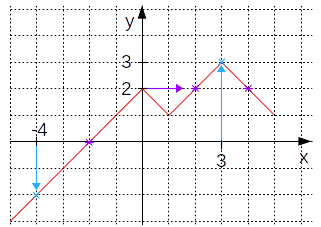
\includegraphics[scale=0.9]{assets/serie_1_exo_1_figure_1.png}
\label{fig:p_s_1_exo1-fig1}
\end{figure}

\begin{itemize}
    \item L'image de 3 par la fonction f est 3.
    \item L'image de -4 par la fonction f est -2.
    \item L'antécédent de 0 est -2.
    \item Les antécédents de 2 sont 0, 2, 4.
    \item Le domaine de définition de la fonction est l'intervalle [-5;5] (on voit que x ne peut prendre que des valeurs entre -5 et 5 sur l'axe des abscisses).
    \item Le domaine image de la fonction est l'intervalle [-3;3] (on remarque que la fonction f prend des valeurs comprises entre -3 et 3 sur l'axe des ordonnées).
\end{itemize}
\noindent\rule{\textwidth}{1pt}

\subsubsection*{Questions:}
Soit les fonctions g et h dont les représentations graphiques sont représentées sur la figure ci-dessous.

\begin{figure}[!h]
\center
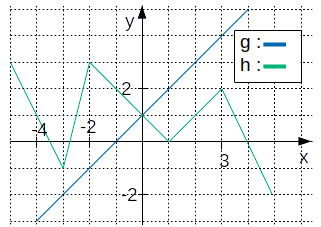
\includegraphics[scale=0.9]{assets/serie_1_exo_1_figure_2.png}
\label{fig:p_s_1_exo1-fig2}
\end{figure}

\begin{enumerate}
    \item  Donner les images de -4, -2, 0 et 3 par les 2 fonctions.
    \item  Donner les antécédents de -2, 0 et 2 pour les 2 fonctions.
    \item  Quels sont les domaines de définition et images des 2 fonctions g et h.
\end{enumerate}
\vspace{3cm}

\section*{Exercice 2: expression algébrique et représentation graphique}
Dans cet exercice, vous allez calculer des images de différentes fonctions à partir des expressions algébriques et tracer leurs représentations graphiques.

\noindent\rule{\textwidth}{1pt}
\subsubsection*{Exemple:}
Soit la fonction f définie sur $\mathbb{R}$:

\begin{equation}\nonumber
\begin{matrix}
    & \mathbb{R}   &             & \mathbb{R} \\
f : &     x& \rightarrow & 3x-5 
\end{matrix}
\end{equation}

Ici vous avez une notation formelle et très mathématiques, mais elle contient toutes les informations. Le premier $\mathbb{R}$ au dessus du $x$ correspond au domaine de définition, le second correspond au domaine image de la fonction.
La variable est $x$ et l'expression algébrique se déduit de l'expression de droite $3x-5$:
$$
f(x) = 3x-5
$$
Si nous désirons connaître l'image de 3 par f, il faut alors substituer (le terme souvent utilisé en maths est injecter) 3 dans l'expression (à la place de x):
\begin{equation}\nonumber
\begin{matrix}
& f(3) & = & 3\times(3) - 5 \\
\Leftrightarrow & f(3) & = & 9 - 5 \\
\Leftrightarrow & f(3) & = & 4
\end{matrix}
\end{equation}
En calculant plusieurs images de la fonction f on peut observer la tendance de ses variations et construire un tableau de valeurs:
\begin{table}[!h]
\center
\begin{tabular}{|c|c|c|c|c|c|c|c|c|}
\hline
  x   & -3  & -2 &-1 &  0 &  1 & 2 & 3  \\ \hline
 f(x) &-14 &-11 &-8 & -5 & -2 & 1 & 4  \\ \hline
\end{tabular}
\end{table}

Ce tableau de valeurs permet ensuite de placer ces points (coordonnées ($x$,$f(x)$)) de la fonction dans un repère:

\begin{figure}[!h]
\center
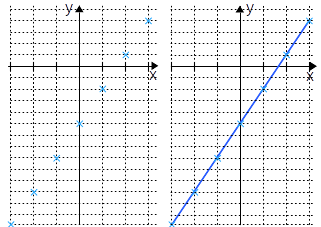
\includegraphics[scale=0.9]{assets/serie_1_exo_2_figure_1.png}
\label{fig:p_s_1_exo2-fig1}
\end{figure}

\noindent\rule{\textwidth}{1pt}

\subsubsection*{Questions:}
Soit les fonctions g et h dont les expressions algébriques sont données ci-dessous:
\begin{equation}\nonumber
\begin{matrix}
& \mathbb{R} & & \mathbb{R} \\
g : & x & \mapsto & -\frac{1}{2}x + 3\\
h : & x & \mapsto & 2x + 1\\
\end{matrix}
\end{equation}

\begin{enumerate}
    \item  Donner l'expression algébrique de la fonction g et de la fonction h.
    \item  Donner le tableau de valeurs de ces 2 fonctions pour x appartenant à:
    $$
    \{-5; -4; -3; -2; -1; -\frac{1}{2}; 0; 1; \frac{3}{2}; 2; 3; 4; 5\}
    $$
    \item  Tracer les représentations graphiques de ces 2 fonctions.
    \item  Par lecture graphique, quelles sont les coordonnées du point d'intersection ?
\end{enumerate}

L'intersection entre 2 courbes de fonctions se caractérise de manière algébrique par l'égalité entre les 2 fonctions:
\begin{equation}\nonumber
h(x_i) = g(x_i)
\end{equation}

On peut alors substituer les fonctions par leurs expressions et simplifier l'équation afin de déterminer la valeur de $x_i$:

\begin{align}
-\frac{1}{2}x_i+3 = 2x_i+1 & \Leftrightarrow -\frac{1}{2}x + 3 -1 = 2x_i + 1 -1 \nonumber\\
& \Leftrightarrow -\frac{1}{2}x + 2 = 2x_i \nonumber\\
& \Leftrightarrow -\frac{1}{2}x + 2 + \frac{1}{2}x_i = 2x_i + \frac{1}{2}x_i \nonumber\\
& \Leftrightarrow 2 = (2+\frac{1}{2})x_i \nonumber\\
& \Leftrightarrow 2 = \frac{5}{2}x_i \nonumber\\
& \Leftrightarrow x_i = 2\times \frac{2}{5} = \frac{4}{5} \nonumber
\end{align}

\begin{enumerate}
    \setcounter{enumi}{4}
    \item Déterminer par le calcul, les coordonnées du point d'intersection (je vous encourage à refaire le calcul vous même).
\end{enumerate}

\subsubsection*{Note:}
Vous vous frotterez plus longuement aux systèmes d'équations lorsque vous serez à la dernière fiche d'analyse.
\vspace{3cm}

\section*{Exercice 3 : Coding time !}
Dans cet exercice vous n'aurez plus besoin de vos crayons et de vos feuilles, il est temps de passer à l'application avec python.

\subsection*{Partie 1: Images}
Comme vous l'avez vu dans le premier exercice, l'antécédent et l'image sont, en très gros (ça va faire mal aux mathématiciens de lire ça), respectivement l'input et l'ouput de la fonction.

Pour calculer les images d'un ensemble X de valeurs, vous savez très probablement le faire.\
Quatre options (au moins) s'offrent à vous:
\begin{itemize}
    \item Les opérations avec les listes,
    \item la compréhension de liste,
    \item la fonction lambda,
    \item les opérations avec les arrays de \textbf{Numpy}.
\end{itemize}

\subsubsection*{Questions:}
Vous devez calculer les images des valeurs au sein de la liste $X$, pour les fonctions suivantes:
\begin{equation}\nonumber
f(x) = 5x -20\\
g(x) = -7x -3 \\
h(x) = \frac{7}{5}x -11
\end{equation}

La liste $X$ est $\{ -10, -9, -8, ..., 8, 9, 10\}$.

\begin{lstlisting}[style=nightly]
funct = lambda x : "expression de la fonction"
Im = map( funct(x) for x in [-2, -1, 0, 1, 2])
\end{lstlisting}
Cette manière de faire sera pertinente lorsque l'on regardera les fonctions à plusieurs variables mais vous pouvez l'utiliser tout de même si vous le souhaitez.

\subsection*{Partie 2: Antécédents}
Si l'on souhaite s'intéresser aux antécédents, c'est, à l'inverse de trouver des images, plus compliqué.

Il vous faut raisonner à partir de l'expression algébrique.

\noindent\rule{\textwidth}{1pt}
\subsubsection*{Exemple:}
Soit la fonction $f_1 = 8x-10$, imaginons que vous souhaitez déterminer la valeur de x pour laquelle la fonction vaut 4.\\
Vous pouvez alors écrire l'équation suivante:
\begin{equation}\nonumber
4 = f_1(x_s)  = 8x_s-10 \\
\Leftrightarrow 4 = 8x_s - 10 \\
\end{equation}
Vous réarrangez ensuite l'équation et obtenez:
\begin{equation}\nonumber
8x_s - 14 = 0 \\
\end{equation}

(soustraction de part et d'autre par 4).\
Vous résolvez ensuite cette équation et vous obtenez $x_s = \frac{7}{4}$.

\noindent\rule{\textwidth}{1pt}

En python, vous pouvez utiliser la librairie \textbf{Numpy} ou \textbf{Sympy} pour résoudre des systèmes d'équations linéaires, notamment avec:
\begin{itemize}
    \item \inlsnippet{linalg.solve()} pour \textbf{Numpy},
    \item \inlsnippet{solve()} ou \inlsnippet{solveset()} pour \textbf{Sympy}.
\end{itemize}


\subsubsection*{Questions:}
Pour cette partie, vous devez pour chacune des fonctions $f$, $g$ et $h$, calculer les antécédents des éléments de la liste:
$$
Y = [-25, 13, -42, 42, 21, 19, 1, 0, 3/2]
$$


\subsubsection*{Remarques:}
Faites cela proprement et coder une fonction qui vous retourne les solutions.\\
Prenez le temps de parcourir la page  sur le \href{https://docs.sympy.org/latest/modules/solvers/solvers.html#algebraic-equations}{solver de Sympy}.\\
\textit{(Vous pourriez être intéressé par le module \inlsnippet{Eq()} de Sympy).}

\subsection*{Partie 3: Représentation graphique}

Enfin, vous allez demander à python de représenter les fonctions que vous souhaitez.\
Pour cela, rien de tel que le module \inlsnippet{matplotlib.pyplot}.

Votre boulot est de représenter l'ensemble des fonctions présentes dans ce sujet, laissez votre côté artiste s'exprimer :
\begin{itemize}

    \item \inlsnippet{plot(X, Y, color = "...", linewidth = ..., marker = ".", ...)}
    \item \inlsnippet{scatter(X, Y, ...)}
    \item \inlsnippet{subplot()}
\end{itemize}

Explorer la page de \href{https://matplotlib.org/3.1.1/gallery/index.html}{mathplotlib}.

%\begin{lstlisting}[style=nightly]
%import numpy as np
%def test_function:
 %   """
 %   Description..
 %   """
 %   for i in range(0,5):
 %       list()
 %       int()
 %       return
 %   
 %   # comment
 %   x = 2
 %   test_function()
%\end{lstlisting}

\end{document}
%%%%%%%%%%%%%%%%%%%%%%%%%%%%%%%%%%%%%%%%%%%%%%%%%%%%%